\documentclass[main]{subfiles}

\begin{document}
    \Date{03.12.19}

    \begin{task}
        Найдите уравнения геодезических кривых на сфере
        \[S^2 = \{(x,y,z) \in \R^3 \ |\ x^2 + y^2 + z^2 = 1\}\]
        двумя способами
    \end{task}

    \begin{Remark}
        \[(0,\ \pi) \times \R \ra \R^3\]
        \[\theta, v \mapsto (\cos \theta,\ \sin \theta,\ v)\]
        \[\RNumb{1} = \begin{pmatrix}
            1 & 0\\
            0 & 1
        \end{pmatrix}\]
        \[\Gamma_{ij}^k = 0\]
        \[\begin{cases}
            \ddot{\theta} = 0 & \theta(t) = \alpha t + \beta\\
            \ddot{v} = 0 & v(t) = \w{\alpha} t + \w{\beta}
        \end{cases}\]
        \begin{figure}[H]
            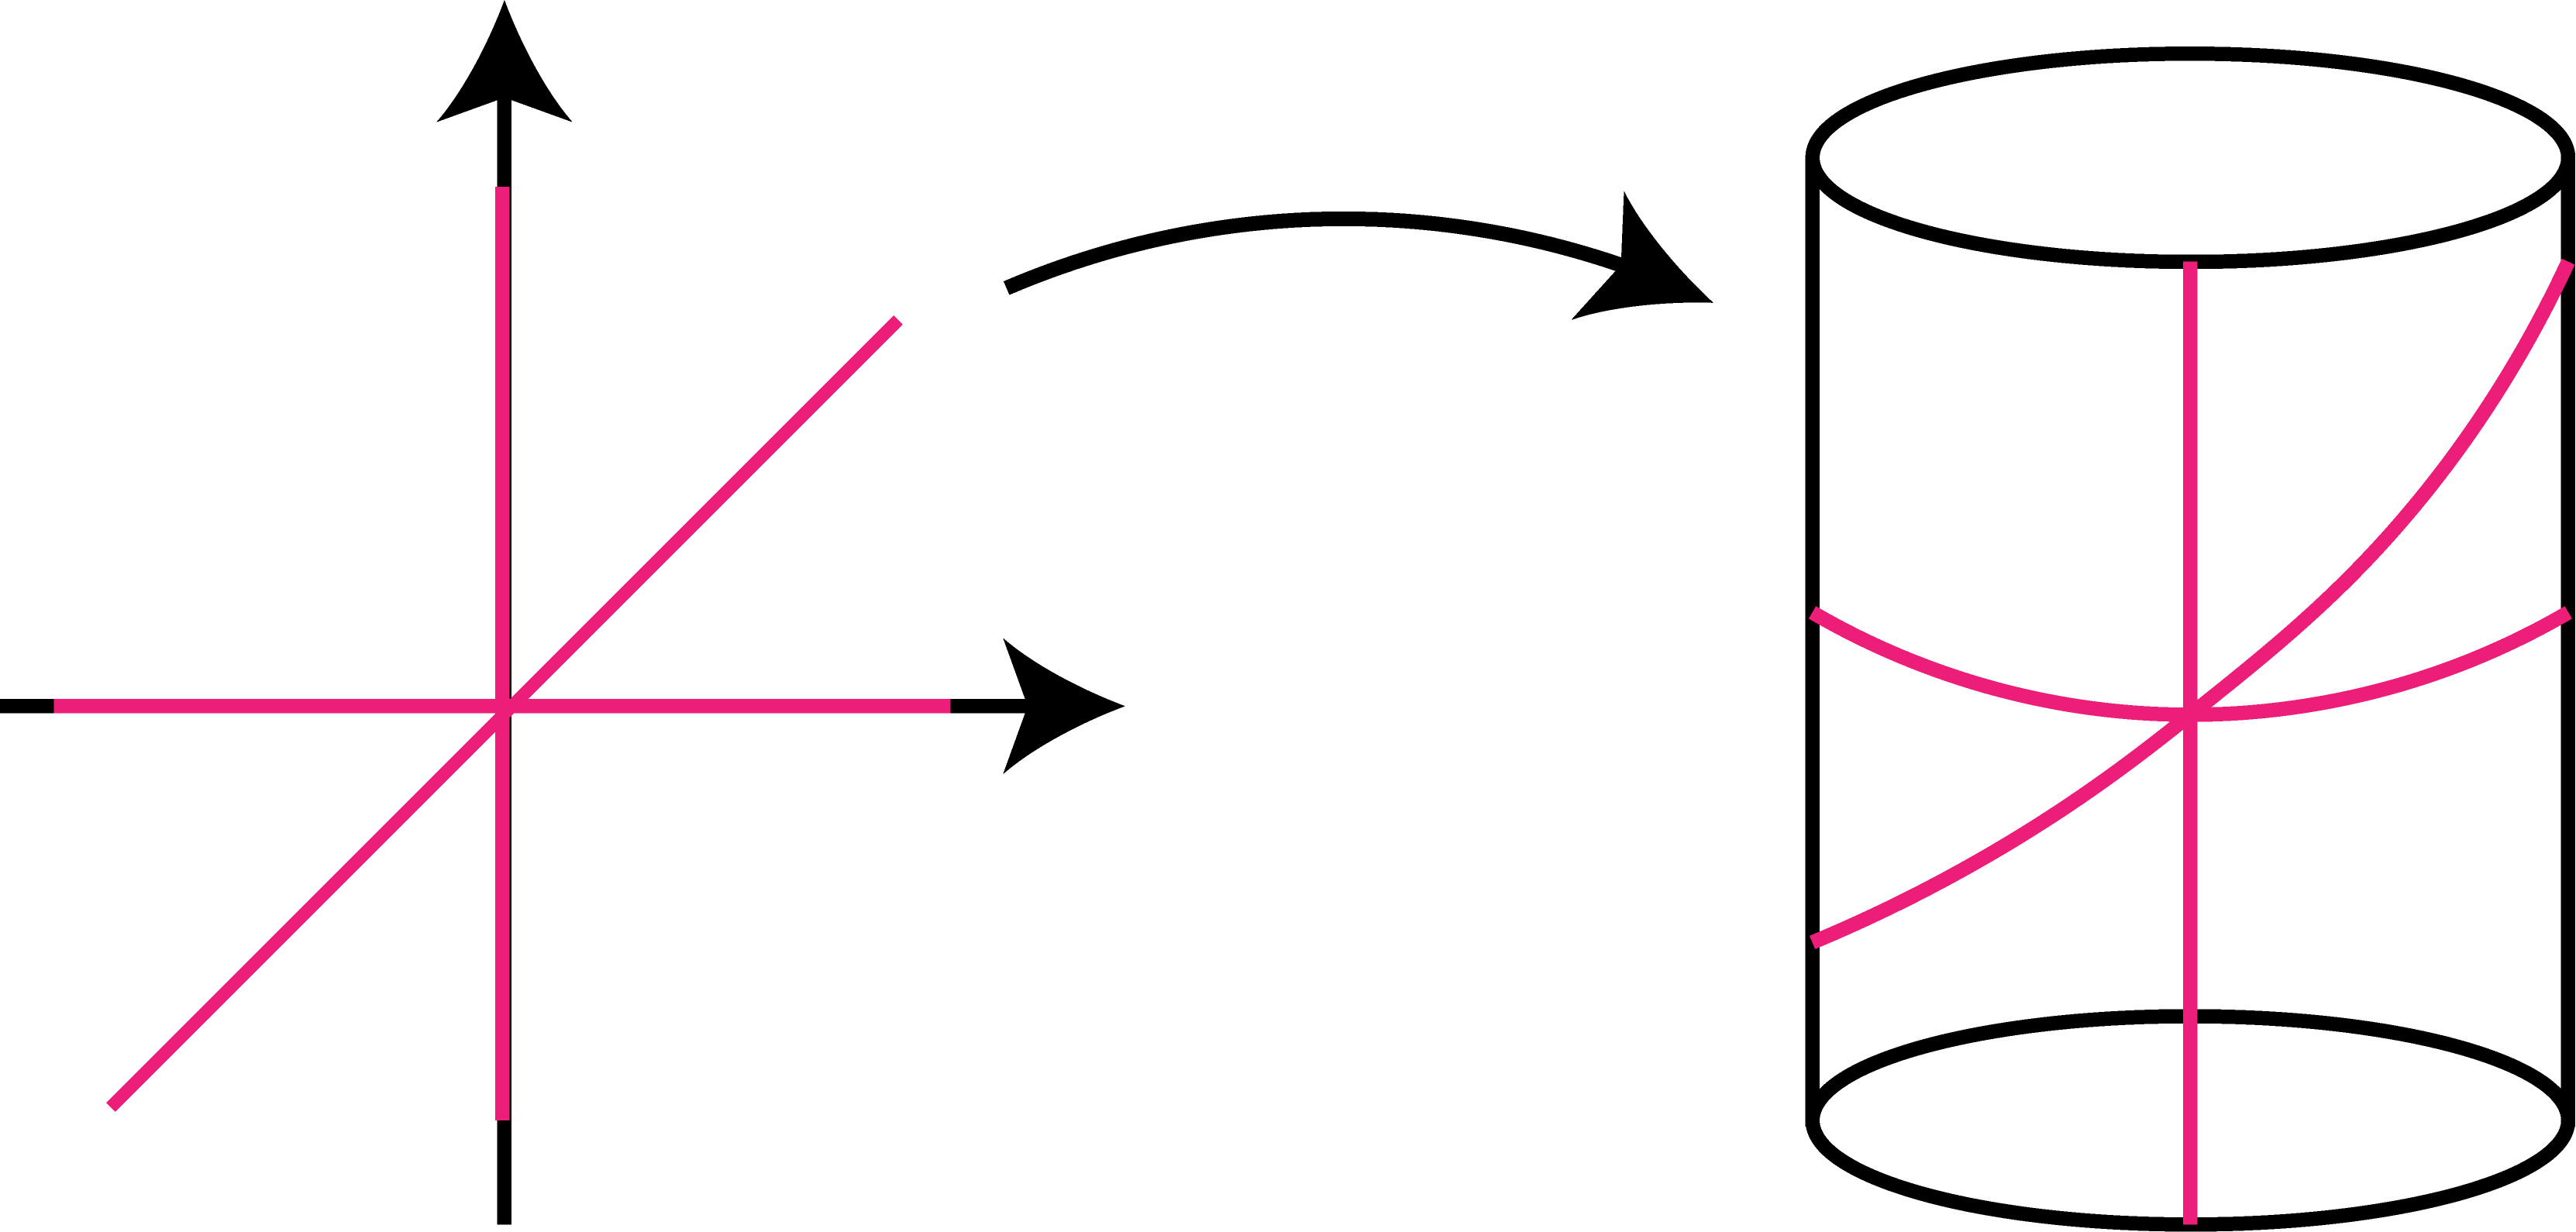
\includegraphics[width=7cm]{pics/14_1}
            \centering
        \end{figure}
    \end{Remark}

    \begin{sol}
        Параметризация для сферы радиуса 1:
        \[\begin{cases}
          x = \cos\theta \cos\varphi\\
          y = \sin\theta \cos\varphi\\
          z =\sin\varphi
        \end{cases}\]
        %Найдем переменные для $\RNumb{1}(F)$:
        %\[<\frac{\d F}{\d \varphi},\ \frac{\d F}{\d \varphi}> = \sin^2 \varphi \sin^2 \theta + \sin^2 \varphi \cos^2 \theta + \cos^2 \varphi = 1\]
        %\[<\frac{\d F}{\d \varphi},\ \frac{\d F}{\d \theta}> = 0,\q <\frac{\d F}{\d \theta},\ \frac{\d F}{\d \varphi}> = 0,\q <\frac{\d F}{\d \theta},\ \frac{\d F}{\d \theta}> = \cos^2 \varphi\]
        \[\Ra \RNumb{1}(F)=\begin{pmatrix}
          1 & 0\\
          0 & \cos^2 \theta
        \end{pmatrix}\]
        Знаем:
        \[\Gamma^1_{11} E + \Gamma_{11}^2 F = \frac{1}{2}E_{\theta}  \qq\qq E_{\theta} = \frac{\d }{\d \theta} E \]
        \[\Gamma^1_{11} F + \Gamma_{11}^2 G = F_{\theta} - \frac{1}{2}E_{\varphi}  \]
        \[\Gamma^1_{12} E + \Gamma_{12}^2 F = \frac{1}{2} E_{\varphi}  \]
        \[\Gamma_{12}^1 F + \Gamma_{12}^2 G = \frac{1}{2} G_{\theta} \]
        \[\Gamma_{22}^1 E + \Gamma_{22}^2 F = F_{\varphi} - \frac{1}{2}G_{\theta}  \]
        \[\Gamma_{22}^1 F + \Gamma_{22}^2 G = \frac{1}{2} G_{\varphi}  \]
        \[\Ra \begin{cases}
            \Gamma^1_{11} = 0\\
            \Gamma_{11}^2 (\cos^2 \theta) = 0\\
            \Gamma^1_{12} = 0\\
            \Gamma_{12}^2 (\cos^2 \theta)  = - \sin \theta \cos \theta\\
            \Gamma_{22}^1 = \sin \theta \cos \theta\\
            \Gamma_{22}^2 (\cos^2 \theta) = 0
        \end{cases} \RA
        \begin{cases}
            \Gamma^1_{11} = 0\\
            \Gamma_{11}^2 = 0\\
            \Gamma^1_{12} = 0\\
            \Gamma_{12}^2 = - \tg \theta\\
            \Gamma_{22}^1 = \sin \theta \cos \theta\\
            \Gamma_{22}^2 = 0
        \end{cases}\]
        \[F: \ub{u}{(0,\ 2\pi) \times (0,\ \pi)} \ra S^2 \subset \R\]
        Напишем:
        \[\ddot{\gamma_k} + \us{i=1}{\os{2}{\sum}} \us{j=1}{\os{2}{\sum}} \Gamma_{ij}^k \dot{\gamma}_i \dot{\gamma}_j = 0\]
        Значит:
        \[\gamma: [0,1] \ra u\]
        \[t \mapsto (\theta(t), \varphi(t))\]
        \[\ddot{\theta} + \us{=0}{\Gamma_{11}^1} \dot{\theta} \dot{\theta} + \us{=0}{\Gamma_{12}^1} \dot{\theta} \dot{\varphi} + \us{=0}{\Gamma_{21}^1} \dot{\varphi} \dot{\theta} + \Gamma_{22}^1 \dot{\varphi} \dot{\varphi} = 0\]
        \[\Ra \ddot{\theta}(t) + \cos \theta(t) \sin (\theta) \dot{\varphi}^2 = 0\]
        \[\ddot{\varphi}(t) + \Gamma_{11}^2 \dot{\theta}^2 + \Gamma_{12}^2 \dot{\theta} \dot{\varphi} + \Gamma_{21}^2 \dot{\varphi} \dot{\theta} + \Gamma_{22}^2 \dot{\varphi} \dot{\varphi} = 0\]
        \[\Ra \ddot{\varphi}(t) - 2\tg(\theta) \dot{\theta} \dot{\varphi} = 0\]
        \begin{figure}[H]
            \centering
            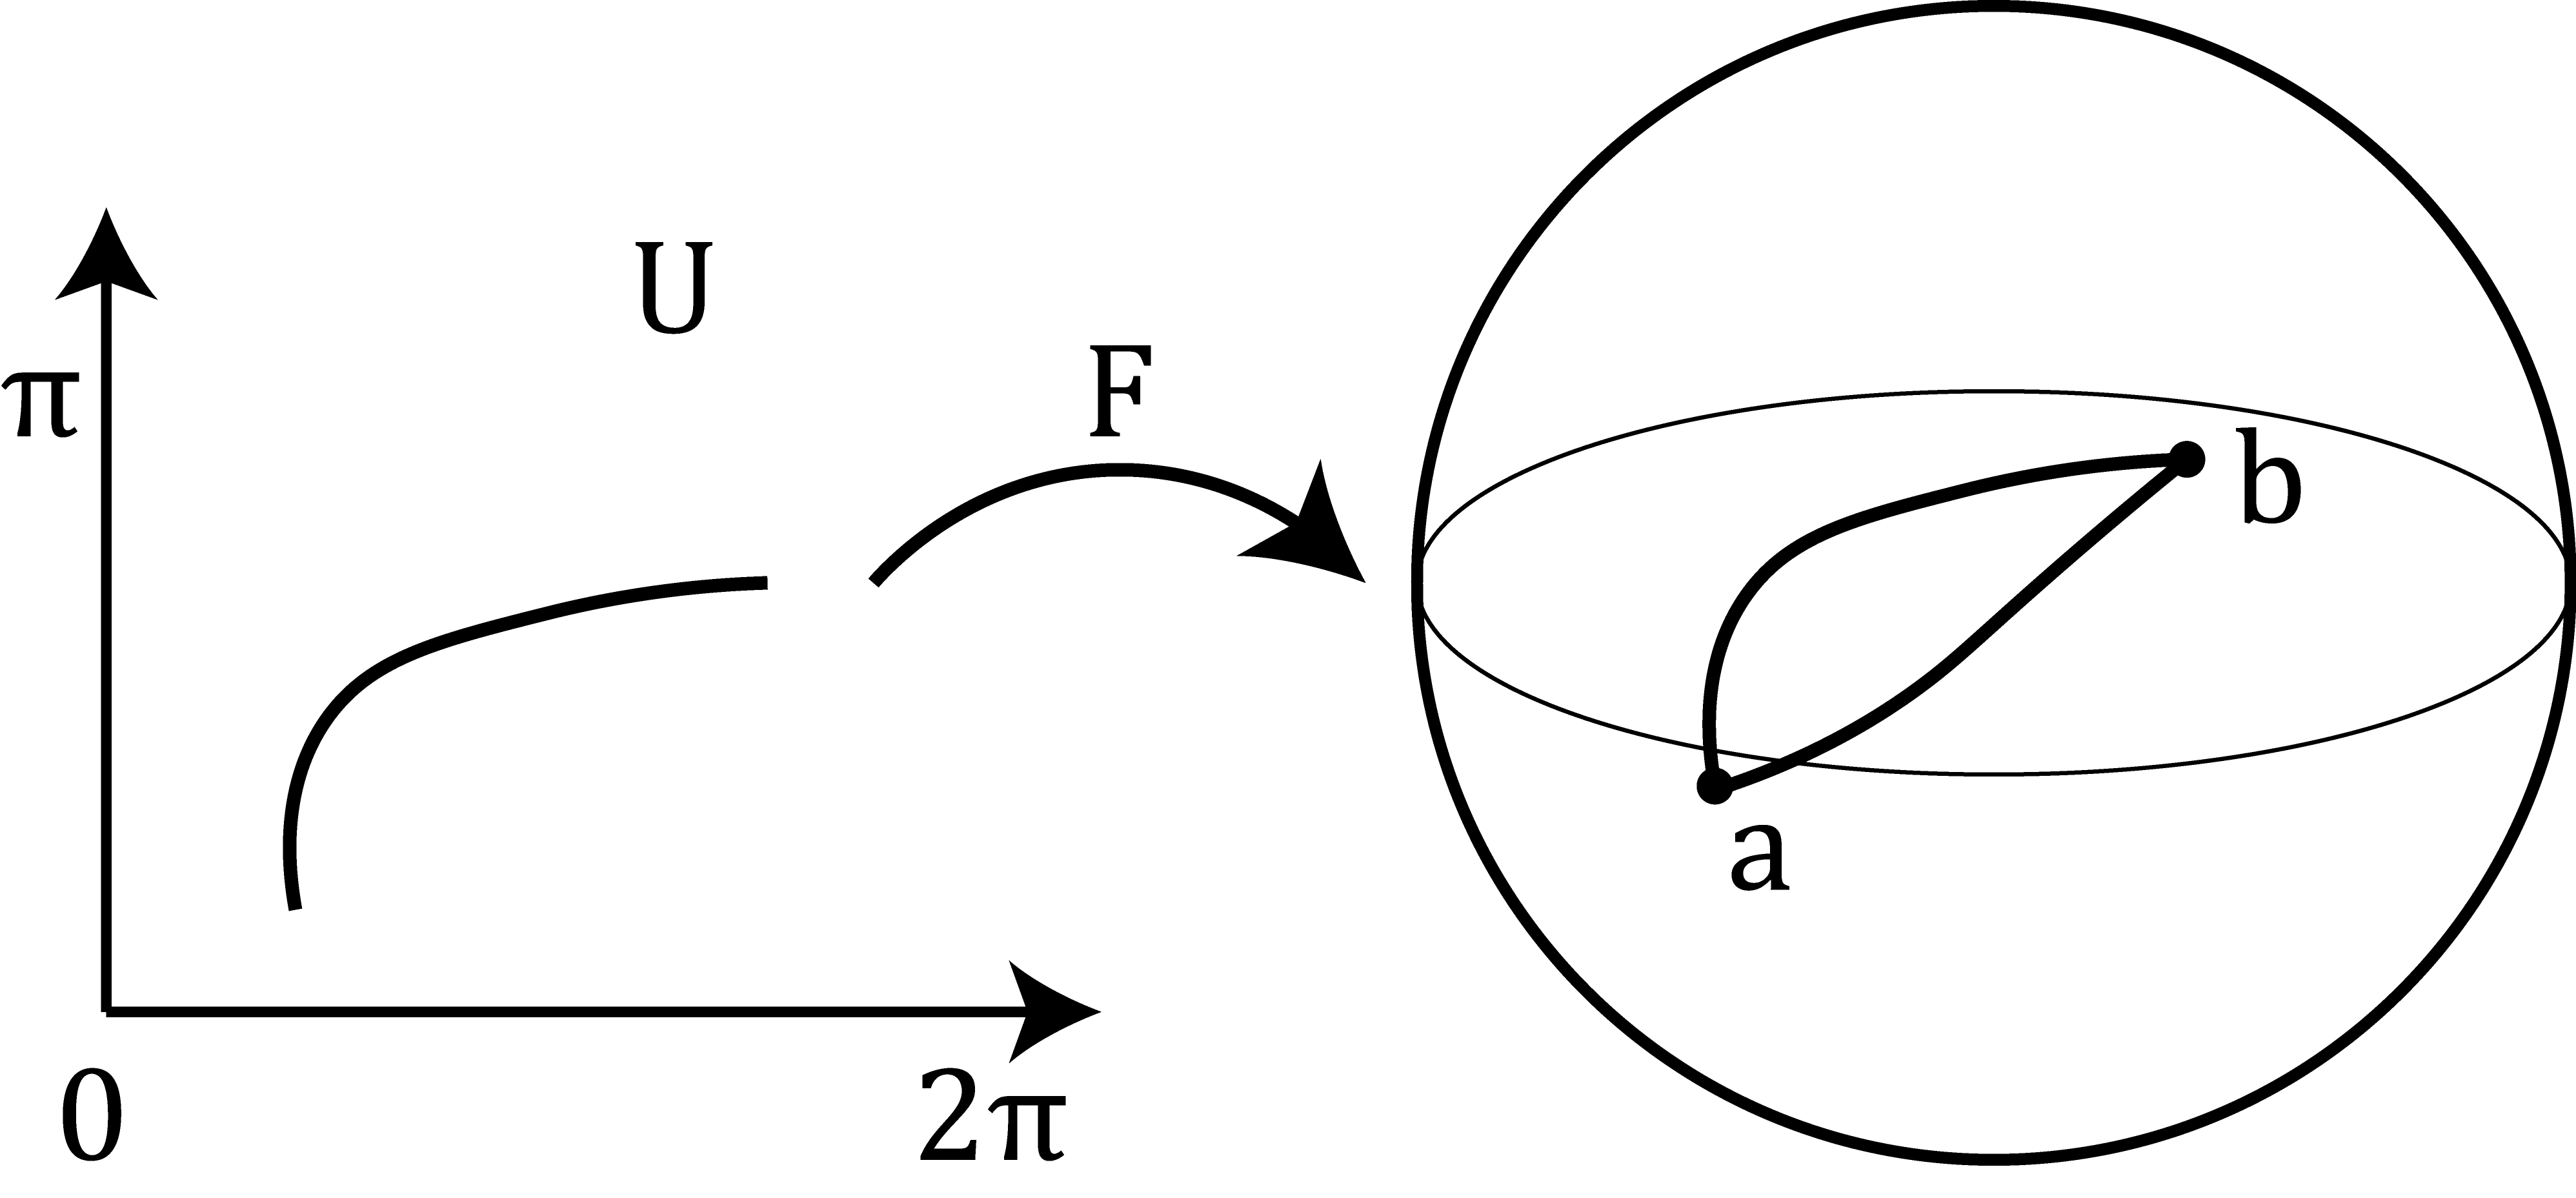
\includegraphics[width=8cm]{pics/14_2}
            \caption{У нас есть сфера с двумя произвольными точками a,b. Хотим найти кривую на сфере L, которая будет минимизировать расстояние. Сводим задачу к плоскости, существует биекция между кривыми}
        \end{figure}
        \[\forall \beta \q \e \gamma: \beta = F \circ \gamma\]
        \[l(\beta) = \int_0^1 \dot{\beta}(t) dt = \int_0^1 |\dot{F \circ \gamma}| dt =\]
        \[= \int_0^1 \sqrt{<\begin{pmatrix}
            \dot{\gamma}_1\\
            \dot{\gamma}_2
        \end{pmatrix}>, \RNumb{1}_{\gamma} \begin{pmatrix}
            \dot{\gamma}_1\\
            \dot{\gamma}_2
        \end{pmatrix}} dt\]
        \[C^{\infty}([0,1],\ u) \ra \R\]
        \[\gamma \mapsto \int_0^1 \sqrt{<\begin{pmatrix}
            \dot{\gamma}_1\\
            \dot{\gamma}_2
        \end{pmatrix}>, \RNumb{1}_{\gamma} \begin{pmatrix}
            \dot{\gamma}_1\\
            \dot{\gamma}_2
        \end{pmatrix}} dt\]
        \[\gamma(t) = (\theta(t),\ \varphi(t))\]
        \[\begin{pmatrix}
            \theta(t)\\
            \varphi(t)
        \end{pmatrix} \mapsto \int_0^1 (\dot{\theta})^2 (t) + \cos^2 (\theta(t) \dot{\varphi}^2 (t))^{\frac{1}{2}} dt\]
        Искать $\min \int |f|^2 dt \ \lra \ $искать $\min \int |f| dt$
        \[\begin{cases}
            \dfrac{d}{dt} \dfrac{\d L}{\d \dot{\theta}} - \dfrac{\d L}{\d \theta} = 0\\ \\
            \dfrac{d}{dt} \dfrac{\d L}{\d \dot{\varphi}} - \dfrac{\d L}{\d \theta} = 0
        \end{cases}\]
        \[\frac{d}{dt} 2 \cos^2 \theta \dot{\varphi} = 2 \cos^2 \theta \ddot{\varphi} - 4 \dot{\theta} \cos \theta \sin \theta \dot{\varphi}\]
        Второе уравнение:
        \[\ddot{\varphi} 2 \cos \theta - 4 \cos \theta \sin \theta \dot{\theta} \dot{\varphi} = 0\]
        \[\lra \ddot{\varphi} - 2 \tg(\theta) \dot{\theta} \dot{\varphi} = 0 \q \cos \theta \neq 0\]
        Первое уравнение такое же
    \end{sol}
\end{document}
